% ME 144L Dynamic Systems & Controls Lab — Lecture Study Guide
\documentclass[9pt,twocolumn]{article}

\usepackage[top=0.5in, bottom=0.5in, left=0.45in, right=0.45in]{geometry}
\usepackage{amsmath,amssymb}
\usepackage{booktabs,array,tabularx}
\usepackage[table]{xcolor}
\usepackage{tikz}
\usetikzlibrary{arrows.meta, positioning, calc}
\usepackage{fancybox}
\usepackage{float}
\usepackage[colorlinks=true, allcolors=blue]{hyperref}

\definecolor{accent}{HTML}{BF5700}
\definecolor{bodytext}{HTML}{333333}
\definecolor{ansbg}{HTML}{FFF8F0}
\definecolor{ansframe}{HTML}{D9A87C}
\definecolor{secbg}{HTML}{F5EDE4}

\color{bodytext}
\pagestyle{empty}
\setlength{\parindent}{0pt}
\setlength{\parskip}{2pt}
\setlength{\columnsep}{12pt}
\setlength{\jot}{2pt}

% compact lists
\setlength{\leftmargini}{1.2em}
\setlength{\itemsep}{0pt}
\setlength{\parsep}{0pt}
\setlength{\topsep}{1pt}

% --- Custom commands ---
\newcommand{\labsec}[1]{%
  \vspace{5pt}%
  \noindent\colorbox{accent}{\parbox{\dimexpr\columnwidth-2\fboxsep}{%
    \centering\bfseries\color{white}\small #1}}%
  \vspace{3pt}\par%
}
\newcommand{\subsec}[1]{%
  \vspace{3pt}%
  {\small\bfseries\textcolor{accent}{#1}}%
  \vspace{1pt}\par\noindent%
}
\newcommand{\eqbox}[1]{%
  \par\noindent\centerline{\fboxsep=3pt\fcolorbox{ansframe}{ansbg}{\parbox{0.92\columnwidth}{\small #1}}}%
  \vspace{2pt}\par%
}
\newcommand{\minibox}[1]{%
  \fboxsep=2pt\fcolorbox{ansframe}{ansbg}{\small\textbf{#1}}%
}

\begin{document}
\small
\setlength{\abovedisplayskip}{2pt}
\setlength{\belowdisplayskip}{2pt}
\setlength{\abovedisplayshortskip}{1pt}
\setlength{\belowdisplayshortskip}{1pt}

\begin{center}
{\Large\bfseries\textcolor{accent}{ME 144L --- Lecture Study Guide}}\\[2pt]
{\normalsize Lectures 2--10 $\mid$ Spring 2026 $\mid$ Alejandro Diaz}
\end{center}
\vspace{2pt}
\hrule height 0.8pt
\vspace{4pt}

% ══════════════════════════════════════════════════════════════
\labsec{Lec 2 --- Signal Processing \& Analysis}
% ══════════════════════════════════════════════════════════════

\subsec{Signal Classification}
\begin{itemize}
  \item \textbf{Physical} (measurable: voltage, force) vs.\ \textbf{non-physical} (computed: stock index)
  \item \textbf{Deterministic} (predictable, repeatable) vs.\ \textbf{Random} (statistical description only)
  \item \textbf{Noise}: unwanted random signal added to desired signal
  \item \textbf{Interference}: unwanted deterministic signal (e.g.\ 60\,Hz hum)
\end{itemize}

\subsec{Statistical Measures}
\eqbox{%
Mean: $\bar{x} = \dfrac{1}{N}\displaystyle\sum_{i=1}^{N} x_i$\\[4pt]
Variance: $\sigma^2 = \dfrac{1}{N-1}\displaystyle\sum (x_i - \bar{x})^2$\\[4pt]
Std.\ dev.: $\sigma = \sqrt{\sigma^2}$\\[3pt]
RMS: $x_{\text{rms}} = \sqrt{\dfrac{1}{N}\displaystyle\sum x_i^2}$
}

\subsec{Sine Wave Measures}
For $x(t) = A\sin(\omega t)$:
\eqbox{%
Peak amplitude: $A$\\[2pt]
RMS value: $A_{\text{rms}} = A/\sqrt{2}$\\[2pt]
Average (full-wave rectified): $\bar{A} = 2A/\pi$
}

\subsec{A/D Conversion}
\eqbox{%
Resolution: $\Delta V = \dfrac{V_{FS}}{2^n}$\\[3pt]
$n$ = number of bits, $V_{FS}$ = full-scale voltage range\\[2pt]
Example: 10-bit, $V_{FS}=5$\,V $\Rightarrow$ $\Delta V = 5/1024 \approx 4.9$\,mV
}

\subsec{Nyquist Sampling Theorem}
\eqbox{%
$f_s \geq 2\,f_{\max}$\\[2pt]
Sampling below Nyquist causes \textbf{aliasing}: high-frequency content folds into lower frequencies and cannot be removed digitally.
}

\textbf{Anti-aliasing filter}: analog (hardware) low-pass filter placed \emph{before} the ADC. Must be analog because aliasing occurs at the sampling stage.

\subsec{First-Order System: Flywheel Spin-Down}
\eqbox{%
$J\,\dot{\omega} = -B\,\omega \;\;\Rightarrow\;\; \omega(t) = \omega_0\,e^{-t/\tau}$\\[3pt]
Time constant: $\tau = J/B$\\[2pt]
At $t = \tau$: $\omega = 0.37\,\omega_0$ \quad (37\% of initial)
}

\subsec{RC Low-Pass Filter}
\eqbox{%
$\tau = RC$, \quad $f_c = \dfrac{1}{2\pi\,RC}$\\[3pt]
Transfer function: $H(s) = \dfrac{1}{\tau s + 1}$
}

\subsec{Digital Filter Design (Bilinear/Tustin Transform)}
Map $s$-domain to $z$-domain:
\eqbox{%
$s = \dfrac{2}{\Delta t}\cdot\dfrac{1 - z^{-1}}{1 + z^{-1}}$\\[4pt]
Yields difference equation:\\
$V_o[k] = -a_1\,V_o[k{-}1] + b_0\,V_i[k] + b_1\,V_i[k{-}1]$
}

Alternatively use \texttt{scipy.signal.cont2discrete} with \texttt{method='zoh'} or \texttt{'bilinear'}.

\subsec{Stationary \& Ergodic Processes}
\begin{itemize}
  \item \textbf{Stationary}: statistical properties (mean, variance) do not change over time
  \item \textbf{Ergodic}: time averages equal ensemble averages --- a single long record is sufficient
\end{itemize}

% ══════════════════════════════════════════════════════════════
\labsec{Lec 3 --- Measurements \& Arduino}
% ══════════════════════════════════════════════════════════════

\subsec{Measurement System Chain}
Physical quantity $\to$ Sensor $\to$ Signal conditioning $\to$ ADC $\to$ Digital processing $\to$ Display/storage

\subsec{Sensor Classification}
\begin{center}
\small
\begin{tabular}{ll}
\toprule
\textbf{Type} & \textbf{Principle}\\
\midrule
Resistive & $R$ changes (strain gage, potentiometer)\\
Capacitive & $C = \varepsilon A/d$ changes (MEMS accel)\\
Inductive & $L$ or mutual inductance changes\\
Piezoelectric & Charge from mechanical stress\\
\bottomrule
\end{tabular}
\end{center}

\subsec{Arduino UNO Specifications}
\begin{itemize}
  \item MCU: ATmega328P, 16\,MHz clock, 5\,V logic
  \item ADC: 10-bit, 6 analog inputs (A0--A5)
  \item 14 digital I/O pins (6 with PWM)
  \item Communication: I$^2$C, SPI, UART
  \item Program structure: \texttt{setup()} runs once, \texttt{loop()} repeats
\end{itemize}

\subsec{Ground Types}
\begin{itemize}
  \item \textbf{Earth ground}: physical connection to earth (safety)
  \item \textbf{Signal/chassis ground}: common reference for circuit voltages
  \item Keep analog and digital grounds separated to reduce noise coupling
\end{itemize}

% ══════════════════════════════════════════════════════════════
\labsec{Lec 4 --- Python DAQ \& Pendulum Modeling}
% ══════════════════════════════════════════════════════════════

\subsec{Simple Pendulum}
\eqbox{%
$J\,\ddot{\theta} = -m\,g\,l\,\sin\theta$\\[3pt]
$J = m\,l^2$, \quad $\omega_n = \sqrt{g/l}$, \quad $T_n = 2\pi/\omega_n$
}

\subsec{Compound Pendulum}
Rigid body pivoting at point $O$ (not the center of mass):
\eqbox{%
$J_O = J_C + m\,l_C^2$ \quad (parallel axis theorem)\\[3pt]
$\omega_n = \sqrt{\dfrac{m\,g\,l_C}{J_O}}$
}
where $J_C$ = moment of inertia about CM, $l_C$ = distance from pivot to CM.

\subsec{Friction Models}
\eqbox{%
Viscous: $\tau_v = B\,\dot{\theta}$ \quad (proportional to speed)\\[2pt]
Coulomb: $\tau_c = \tau_0\,\text{sign}(\dot{\theta})$ \quad (constant magnitude)\\[3pt]
Combined: $\tau_f = B\,\dot{\theta} + \tau_0\,\text{sign}(\dot{\theta})$
}

\begin{itemize}
  \item Viscous damping $\to$ exponential amplitude decay
  \item Coulomb friction $\to$ linear amplitude decay
\end{itemize}

\subsec{Potentiometer Voltage Divider}
\eqbox{%
$V_{\text{out}} = V_s \cdot \dfrac{R_2}{R_1 + R_2}$
}

\subsec{Linear Sensor Calibration}
$y_m = K \cdot V_m + b$\\[2pt]
$K$ = sensitivity (slope), $b$ = offset. Determined by linear regression of known inputs vs.\ sensor output.

\subsec{Resistance \& Resistivity}
$R = \rho\,L/A$\\[2pt]
$\rho$ = resistivity, $L$ = length, $A$ = cross-sectional area.

% ══════════════════════════════════════════════════════════════
\labsec{Lec 5 --- Beam Vibration \& Accelerometers}
% ══════════════════════════════════════════════════════════════

\subsec{Accelerometer Types}
\begin{center}
\small
\begin{tabular}{ll}
\toprule
\textbf{Type} & \textbf{Mechanism}\\
\midrule
Piezoelectric & Charge from crystal deformation\\
Piezoresistive & Strain gages on deflecting beam\\
Capacitive & Gap change $\to$ $C = \varepsilon A/d$\\
\bottomrule
\end{tabular}
\end{center}

Capacitive MEMS accelerometers (like ADXL05) model the proof mass as a mass--spring--damper system. They respond down to DC (can measure gravity).

\subsec{LSM6DSO 6-DOF IMU}
\begin{itemize}
  \item Accelerometer: $\pm 2/4/8/16\,g$, sensitivity $0.061~\text{mg/LSB}$ at $\pm 2g$
  \item Gyroscope: $\pm 125$ to $\pm 2000~\text{dps}$
  \item Interface: I$^2$C or SPI
  \item \textbf{2g test}: rotate sensor $\pm 1g \to \mp 1g$ to verify $2g$ total change and confirm sensitivity
\end{itemize}

\subsec{Cantilever Beam Stiffness}
\eqbox{%
$k = \dfrac{3\,E\,I}{L^3}$, \qquad $I = \dfrac{b\,h^3}{12}$\\[4pt]
$E$ = Young's modulus, $b$ = width, $h$ = thickness, $L$ = free length
}

\subsec{Natural Frequency of Beam--Mass System}
\eqbox{%
Massless beam: $\omega_{n} = \sqrt{k/M}$\\[2pt]
With beam mass: $\omega_n = \sqrt{\dfrac{k}{M + 0.23\,m_{\text{beam}}}}$
}
The factor 0.23 accounts for the distributed mass of the cantilever contributing to the effective vibrating mass.

\subsec{Damped Free Vibration Response}
\eqbox{%
$x(t) = A_0\,e^{-\zeta\omega_n t}\cos(\omega_d\,t - \phi)$\\[3pt]
$\omega_d = \omega_n\sqrt{1 - \zeta^2}$, \quad $T_d = 2\pi/\omega_d$
}

\subsec{Log Decrement Method}
Plot $\ln(A_0/A_n)$ vs.\ cycle number $n$:
\eqbox{%
Slope: $\beta = \dfrac{2\pi\zeta}{\sqrt{1-\zeta^2}}$\\[4pt]
$\zeta = \dfrac{\beta}{\sqrt{4\pi^2 + \beta^2}}$\\[4pt]
Light damping: $\beta \approx 2\pi\zeta$
}

\begin{itemize}
  \item Linear $\ln(A_0/A_n)$ vs.\ $n$ $\Rightarrow$ linear (viscous) damping
  \item Nonlinear trend $\Rightarrow$ Coulomb (nonlinear) damping
\end{itemize}

% ══════════════════════════════════════════════════════════════
\labsec{Lec 6 --- Strain Gages \& Force Measurement}
% ══════════════════════════════════════════════════════════════

\subsec{Strain Gage Fundamentals}
\eqbox{%
Gage factor: $G = \dfrac{1}{\varepsilon}\dfrac{\Delta R}{R} = (1 + 2\nu) + \dfrac{1}{\varepsilon}\dfrac{\Delta\rho}{\rho}$\\[4pt]
Resistance change: $\Delta R = G\cdot\varepsilon\cdot R$
}
$\varepsilon$ = strain, $\nu$ = Poisson's ratio.\\
First term $(1+2\nu)$: geometric effect. Second term: piezoresistive effect.\\
Typical metal foil gage: $G \approx 2$.

\subsec{Wheatstone Bridge}
\eqbox{%
$V_o = V_s\!\left(\dfrac{R_1 R_4 - R_2 R_3}{(R_1+R_2)(R_3+R_4)}\right)$\\[4pt]
Equal-arm with active gages:\\
$\dfrac{\Delta V_o}{V_s} = \dfrac{G}{4}\left(\varepsilon_1 - \varepsilon_2 + \varepsilon_3 - \varepsilon_4\right)$
}

Bridge is balanced ($V_o = 0$) when $R_1 R_4 = R_2 R_3$.

\subsec{Bridge Configurations}
\begin{center}
\small
\begin{tabular}{lcc}
\toprule
Config & Active gages & Bridge constant $K$\\
\midrule
Quarter & 1 & 1\\
Half & 2 & 2\\
Full & 4 & 4\\
\bottomrule
\end{tabular}
\end{center}
Full bridge: $\Delta V_o / V_s = G\,\varepsilon$. Higher $K$ gives greater sensitivity and cancels temperature drift.

\subsec{Bending Strain in a Cantilever}
\eqbox{%
$\varepsilon = \dfrac{M\,c}{E\,I}$, \quad $I = \dfrac{b\,h^3}{12}$\\[3pt]
$M$ = bending moment, $c = h/2$ = distance to neutral axis
}

Top and bottom surfaces have equal and opposite strains $\to$ ideal for half/full bridge with gages on both sides.

\subsec{Signal Conditioning Chain}
Strain $\to$ $\Delta R$ (via gage factor) $\to$ Bridge unbalance ($\Delta V_o$) $\to$ Amplifier $\to$ ADC

\subsec{NAU7802 24-bit ADC}
High-resolution ADC for load cell applications. Sample rates: 10--320\,SPS. 24-bit resolution gives $V_{FS}/2^{24}$ per count.

% ══════════════════════════════════════════════════════════════
\labsec{Lec 7 --- Two-Can Fluid System}
% ══════════════════════════════════════════════════════════════

\subsec{Hydraulic Capacitance}
A tank stores fluid energy via height (pressure):
\eqbox{%
$C = \dfrac{A}{\rho\,g}$, \quad $P = \rho\,g\,h = \dfrac{V}{C}$\\[3pt]
$A$ = cross-section area. Larger $A \to$ larger $C \to$ slower draining.
}

\subsec{Orifice Flow (Bernoulli-Derived)}
\eqbox{%
$Q = C_c\,A_o\sqrt{\dfrac{2P}{\rho}} = C_c\,A_o\sqrt{2g\,h}$\\[4pt]
$C_c = A_{\text{jet}}/A_o$ (contraction coefficient)\\[2pt]
$C_v = v_{\text{actual}}/v_{\text{ideal}}$ (velocity coefficient)
}

Bernoulli with area ratio:
$v_2 = \sqrt{\dfrac{2g\,h}{1 - (A_2/A_1)^2}}$

\subsec{Volume-Based Outflow Model}
\eqbox{%
$Q = K\sqrt{V}$, \quad $K = A_o\sqrt{\dfrac{2g}{A_{\text{can}}}}$ (ideal)
}

\subsec{Experimental $K$ from Emptying Test}
\eqbox{%
$2\sqrt{V_o} = K\cdot T_e$\\[2pt]
$K = \dfrac{2\sqrt{V_o}}{T_e}$
}

\subsec{One-Can ODE}
$\dot{V} = Q_{\text{in}} - K\sqrt{V}$

\subsec{Two-Can System ODEs}
\eqbox{%
$\dot{V}_1 = -K_1\sqrt{V_1}$\\[3pt]
$\dot{V}_2 = K_1\sqrt{V_1} - K_2\sqrt{V_2}$\\[3pt]
Equilibrium: $K_1\sqrt{V_1^*} = K_2\sqrt{V_2^*}$
}

Nonlinear system --- solved numerically with RK4.

% ══════════════════════════════════════════════════════════════
\labsec{Lec 8 --- Vision-Based Measurement}
% ══════════════════════════════════════════════════════════════

\subsec{Machine Vision Pipeline}
Sensing $\to$ Preprocessing $\to$ Segmentation $\to$ Description $\to$ Recognition $\to$ Interpretation

\subsec{Image Fundamentals}
\begin{itemize}
  \item OpenCV reads in \textbf{BGR} (not RGB) by default
  \item Grayscale: 8-bit $\to$ 256 intensity levels (0 = black, 255 = white)
  \item Convert: \texttt{cv2.cvtColor(img, cv2.COLOR\_BGR2GRAY)}
\end{itemize}

\subsec{Image Sensors: CCD vs.\ CMOS}
\begin{center}
\small
\begin{tabular}{lcc}
\toprule
 & CCD & CMOS\\
\midrule
Quality & Higher & Lower\\
Power & Higher & Lower\\
Integration & Dedicated fab & Standard fab\\
Speed & Slower readout & Faster readout\\
\bottomrule
\end{tabular}
\end{center}

CCD: photodiode $\to$ charge transfer $\to$ amplifier (off-chip).\\
CMOS: per-pixel amplifier, better on-chip processing.

\subsec{Thresholding}
\texttt{cv2.threshold(src, thresh, maxVal, type)}

Types: \texttt{THRESH\_BINARY}, \texttt{THRESH\_BINARY\_INV}, \texttt{THRESH\_TRUNC}, \texttt{THRESH\_TOZERO}.

\subsec{Hough Circle Transform}
\texttt{cv2.HoughCircles(gray, HOUGH\_GRADIENT, dp, minDist, param1, param2, minRadius, maxRadius)}

Detects circles in edge-detected images by voting in parameter space $(x_c, y_c, r)$.

\subsec{Contour Detection \& Object Tracking}
\begin{enumerate}
  \item Select ROI: \texttt{cv2.selectROI()}
  \item Crop frame to ROI
  \item Grayscale $\to$ binary threshold
  \item \texttt{cv2.findContours()} $\to$ largest contour by area
  \item \texttt{cv2.minEnclosingCircle()} $\to$ centroid $(x,y)$
  \item Record $(x, y, t)$ per frame for trajectory
\end{enumerate}

\subsec{Frame Rate \& Timing}
Webcam $\approx$ 30\,fps nominal. Actual rate may vary.\\
Options: constant FPS ($t = i/\text{FPS}$), \texttt{CAP\_PROP\_POS\_MSEC}, or \texttt{time.time()}.

% ══════════════════════════════════════════════════════════════
\labsec{Lec 9 --- PMDC Motor Drives \& Sensing}
% ══════════════════════════════════════════════════════════════

\subsec{PMDC Motor Model Parameters}
Three key parameters for steady-state model:
\begin{center}
\small
\begin{tabular}{lll}
\toprule
Param & Description & How to measure\\
\midrule
$R_m$ & Armature resistance & Ohmmeter\\
$r_m$ & Motor constant & $V_m$ vs $\omega_m$ slope\\
$B_m$ & Viscous damping & $\tau_m$ vs $\omega_m$ slope\\
\bottomrule
\end{tabular}
\end{center}

\subsec{Gyrator Relations}
\eqbox{%
$\tau_m = r_m\,i_m$ \quad (torque $\leftrightarrow$ current)\\[2pt]
$V_m = r_m\,\omega_m$ \quad (back-EMF $\leftrightarrow$ speed)\\[3pt]
$P_{\text{elec}} = V_m\,i_m = \tau_m\,\omega_m = P_{\text{mech}}$
}

\subsec{Back-EMF and Motor Constant}
\eqbox{%
$V_m = V_{in} - R_m\,i_m$\\[3pt]
$r_m = \text{slope of } V_m \text{ vs } \omega_m$ (linear regression)
}

Assumes steady state ($L\,di/dt = 0$).

\subsec{Friction Model}
At no-load steady state, motor torque = friction:
\eqbox{%
$\tau_m = r_m\,i_m = B_m\,\omega_m + \tau_{cf}$\\[3pt]
$B_m$ = slope, $\tau_{cf}$ = intercept of $\tau_m$ vs.\ $\omega_m$
}

\subsec{Torque--Speed Curve}
\eqbox{%
Motor shaft:\\
$\tau_o = \dfrac{r_m}{R_m}\,V_{in} - \left(\dfrac{r_m^2}{R_m} + B_m\right)\omega_m$\\[6pt]
Output shaft (with gearbox):\\
$\tau_o(\omega_o) = GR\,\dfrac{r_m}{R_m}\,V_{in} - GR^2\!\left(\dfrac{r_m^2}{R_m} + B_m\right)\omega_o$\\[4pt]
Stall torque: $\tau_s = GR\,\dfrac{r_m}{R_m}\,V_{in}$\\[3pt]
No-load speed: $\omega_{NL} = \dfrac{r_m\,V_{in}}{r_m^2 + R_m\,B_m}$
}
Increasing $V_{in}$ shifts curves upward (parallel lines).

\subsec{Gear Ratio Calculation}
\eqbox{%
$GR = \dfrac{\omega_m}{\omega_o}$, \quad $\tau_o = GR\cdot\tau_m$\\[3pt]
From tooth counts: $GR = \prod\dfrac{\text{driven}}{\text{driver}}$\\[2pt]
DG01D-E: $GR = 45$
}

\subsec{PWM and H-Bridge}
\eqbox{%
$V_{in} = \dfrac{\text{PWM}}{255}\cdot V_b$
}

\begin{itemize}
  \item H-bridge converts DC bus voltage to modulated drive signal
  \item TB6612FNG: 2-channel driver; IN1/IN2 select CW, CCW, brake, stop
  \item Average voltage to motor $\approx$ duty cycle $\times$ $V_b$
\end{itemize}

\subsec{Encoders}
\begin{center}
\small
\begin{tabular}{lcc}
\toprule
 & Incremental & Absolute\\
\midrule
Output & Pulse train & Coded position\\
Reference & Relative & Absolute\\
Direction & Needs 2 channels & Built-in\\
Cost & Lower & Higher\\
\bottomrule
\end{tabular}
\end{center}

\textbf{Magnetic encoder}: Hall-effect sensors detect rotating magnet. 12\,CPR (counts per revolution) of motor shaft. Output shaft: $12 \times GR$ counts/rev.

\textbf{Quadrature encoding}: two channels (A, B) $90^\circ$ out of phase. Leading channel indicates rotation direction.

\subsec{Arduino Interrupts for Encoders}
\texttt{attachInterrupt(pin, function, RISING)}\\
Set in \texttt{setup()}, not \texttt{loop()}. Pin 0 (digital 2) or pin 1 (digital 3). Arduino timers (16\,MHz crystal $\to$ 62.5\,ns resolution) time transitions between encoder pulses.

% ══════════════════════════════════════════════════════════════
\labsec{Lec 10 --- PMDC Motor Speed Control}
% ══════════════════════════════════════════════════════════════

\subsec{Open-Loop vs.\ Closed-Loop Control}
\begin{center}
\small
\begin{tabular}{lcc}
\toprule
 & Open-Loop & Closed-Loop\\
\midrule
Uses feedback? & No & Yes\\
Model needed? & Yes & Optional\\
Disturbance & Uncompensated & Rejected\\
Complexity & Low & Higher\\
Stability risk & None & Possible\\
\bottomrule
\end{tabular}
\end{center}

\subsec{Open-Loop Motor Control}
Two approaches to determine $G_{OL}$:
\begin{enumerate}
  \item \textbf{Empirical}: fit $\text{PWM} = K_m\,\omega_m + \text{const}$ from experimental data
  \item \textbf{Model-based}: invert torque-speed curve:
\end{enumerate}
\eqbox{%
$V_{in}(\omega_d) = r_m\,\omega_d + \dfrac{R_m}{r_m}\!\left[B_m\,\omega_d + \tau_{c}\tanh(\omega_d)\right]$\\[4pt]
$\text{PWM} = 255 \cdot V_{in}/V_b$
}
OL does not compare output to reference --- susceptible to disturbances and parameter drift.

\subsec{Closed-Loop Feedback Control}

\begin{center}
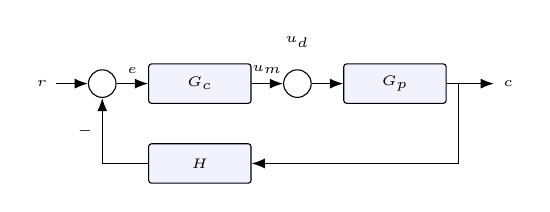
\begin{tikzpicture}[
    node distance=0.9cm and 0.65cm,
    block/.style={draw, rectangle, rounded corners=1pt, minimum width=1.3cm, minimum height=0.5cm, align=center, fill=blue!5, font=\tiny},
    sum/.style={draw, circle, minimum size=0.35cm, inner sep=0pt, font=\tiny},
    >=Latex,
    font=\tiny,
]
    \node (ref)  at (0,0)                       {$r$};
    \node[sum,   right=0.4cm of ref]     (sum1) {};
    \node[block, right=0.4cm of sum1]    (ctrl) {$G_c$};
    \node[sum,   right=0.4cm of ctrl]    (sum2) {};
    \node[block, right=0.4cm of sum2]    (plant){$G_p$};
    \node       [right=0.6cm of plant]   (out)  {$c$};
    \node[block, below=0.5cm of ctrl]    (sens) {$H$};
    \node       [above=0.15cm of sum2]         {$u_d$};

    \draw[->] (ref)    -- (sum1) node[midway, above] {};
    \draw[->] (sum1)   -- (ctrl) node[midway, above] {$e$};
    \draw[->] (ctrl)   -- (sum2) node[midway, above] {$u_m$};
    \draw[->] (sum2)   -- (plant);
    \draw[->] (plant)  -- (out);
    \draw[->] ($(plant.east)+(0.15,0)$) |- (sens);
    \draw[->] (sens)   -| (sum1) node[near end, left] {$-$};
\end{tikzpicture}
\end{center}

Error: $e = r - y_s$, where $y_s = H \cdot c$ is the sensor feedback.

\subsec{Closed-Loop Advantages \& Disadvantages}
\textbf{Advantages}:
\begin{itemize}
  \item Disturbance rejection
  \item Reduced sensitivity to parameter variations
  \item Dynamic tracking via error signal
  \item Enhanced accuracy
\end{itemize}
\textbf{Disadvantages}:
\begin{itemize}
  \item Can lead to oscillation or instability
  \item Requires tuning and/or model for controller design
  \item Sensor failure $\to$ no feedback $\to$ system fails
\end{itemize}

\subsec{PID Control Actions}
\eqbox{%
$u(t) = K_p\,e + K_i\!\displaystyle\int e\,dt + K_d\,\dfrac{de}{dt}$\\[6pt]
\textbf{P}: proportional to error; fast response\\
\textbf{I}: eliminates steady-state error; can reduce stability\\
\textbf{D}: adds effective damping; improves stability
}

\subsec{Digital PID Implementation}
\eqbox{%
$e(k) = r(k) - x(k)$\\[3pt]
$u_p(k) = K_p\,e(k)$\\[2pt]
$u_i(k) = K_i\displaystyle\sum_{j=1}^{k}\dfrac{e(j) + e(j{-}1)}{2}$ \quad (trapezoidal)\\[4pt]
$u_d(k) = -K_d\,[x(k) - x(k{-}1)]$\\[3pt]
$u(k) = u_p(k) + u_i(k) + u_d(k)$
}
Note: $\Delta t$ can be absorbed into gains or kept explicit. Derivative acts on measurement (not error) to avoid kick on setpoint changes.

\subsec{Motor Dynamic ODE (Simulation)}
\eqbox{%
$J_m\,\dot{\omega}_m = -B_m\,\omega_m - \tau_{mo}\,\text{sgn}(\omega_m) + r_m\,i_m$\\[3pt]
$i_m = (V_{in} - r_m\,\omega_m)/R_m$\\[3pt]
$\dot{\theta}_m = \omega_m$, \quad $\theta_s = \theta_m / GR$
}

States: $[\omega_m, \theta_m]$. Inductance ignored ($L_m$ small).

\subsec{Feedforward + PID (FF+PID)}
\eqbox{%
$u = u_{FF} + u_{PID}$\\[3pt]
$u_{FF}$: from OL model (torque-speed inversion)\\
$u_{PID}$: corrects model error and disturbances
}

Feedforward does the ``heavy lifting'' using the model. PID compensates only the residual error, reducing the burden on the integral term.

\subsec{PWM Saturation \& Integrator Windup}
PWM is bounded to $[0, 255]$ (or $[-255, 255]$ for bidirectional). If the controller output exceeds this, the actuator saturates.

\textbf{Windup}: while saturated, the integral term keeps accumulating $\to$ overshoot when the system returns to the linear range. Mitigation: clamp the integral sum or use anti-windup logic.

\subsec{Arduino CL Implementation}
\begin{verbatim}
w_error = wm_ref - wm;
edt = esum + w_error*dtval/1e6;
esum = edt;
dedt = (w_error - elast)/(dtval/1e6);
elast = w_error;
motorPwm = ol_gain*wm_ref
         + kp*w_error + ki*edt + kd*dedt;
\end{verbatim}

% ══════════════════════════════════════════════════════════════
\labsec{Cross-Cutting: 2nd-Order System}
% ══════════════════════════════════════════════════════════════

\subsec{Standard Form}
$m\ddot{x} + c\dot{x} + kx = F(t)$

Normalized: $\ddot{x} + 2\zeta\omega_n\dot{x} + \omega_n^2 x = F/m$

\eqbox{%
$\omega_n = \sqrt{k/m}$, \quad $\zeta = \dfrac{c}{2\sqrt{km}}$, \quad $\omega_d = \omega_n\sqrt{1-\zeta^2}$
}

\begin{center}
\small
\begin{tabular}{lcl}
\toprule
Regime & $\zeta$ & Response\\
\midrule
Underdamped & $0 < \zeta < 1$ & Decaying oscillation\\
Critically damped & $\zeta = 1$ & Fastest non-oscillatory\\
Overdamped & $\zeta > 1$ & Slow exponential return\\
\bottomrule
\end{tabular}
\end{center}

% ══════════════════════════════════════════════════════════════
\labsec{Cross-Cutting: RK4 Integrator}
% ══════════════════════════════════════════════════════════════

For $\dot{x} = f(x,t)$ with step $h$:
\eqbox{%
$k_1 = f(x_i,\, t_i)$\\
$k_2 = f(x_i + k_1 h/2,\, t_i + h/2)$\\
$k_3 = f(x_i + k_2 h/2,\, t_i + h/2)$\\
$k_4 = f(x_i + k_3 h,\, t_i + h)$\\[4pt]
$x_{i+1} = x_i + \dfrac{h}{6}(k_1 + 2k_2 + 2k_3 + k_4)$
}

% ══════════════════════════════════════════════════════════════
\labsec{Quick Reference}
% ══════════════════════════════════════════════════════════════

\begin{center}
\renewcommand{\arraystretch}{1.3}
\small
\begin{tabular}{p{2.6cm}l}
\toprule
\textbf{Quantity} & \textbf{Formula}\\
\midrule
ADC resolution & $V_{FS}/2^n$\\
Nyquist & $f_s \geq 2\,f_{\max}$\\
RC cutoff & $f_c = 1/(2\pi RC)$\\
Flywheel $\tau$ & $J/B$\\
Simple pend.\ $\omega_n$ & $\sqrt{g/l}$\\
Compound pend.\ $\omega_n$ & $\sqrt{mgl_C/J_O}$\\
Beam stiffness & $3EI/L^3$\\
Effective mass & $M + 0.23\,m_{\text{beam}}$\\
Gage factor & $G = (\Delta R/R)/\varepsilon$\\
Bridge (full) & $\Delta V_o/V_s = G\varepsilon$\\
Bending strain & $\varepsilon = Mc/(EI)$\\
Hyd.\ capacitance & $C = A/(\rho g)$\\
Orifice flow & $Q = K\sqrt{V}$\\
Experimental $K$ & $2\sqrt{V_o}/T_e$\\
Motor constant & $r_m = \Delta V_m/\Delta\omega_m$\\
Back-EMF & $V_m = V_{in} - R_m\,i_m$\\
Motor torque & $\tau_m = r_m\,i_m$\\
Torque--speed & $(r_m/R_m)V_{in} - (r_m^2/R_m{+}B_m)\omega_m$\\
Gear ratio & $\omega_o = \omega_m/GR$\\
PWM voltage & $V_{in} = (\text{PWM}/255)\cdot V_b$\\
PID output & $K_p e + K_i\!\int\!e\,dt + K_d\,\dot{e}$\\
Log dec.\ slope & $\beta = 2\pi\zeta/\sqrt{1-\zeta^2}$\\
Damping ratio & $\zeta = \beta/\sqrt{4\pi^2+\beta^2}$\\
Damped freq. & $\omega_d = 2\pi/T_d$\\
Natural freq. & $\omega_n = \omega_d/\sqrt{1-\zeta^2}$\\
RMS (sine) & $A/\sqrt{2}$\\
\bottomrule
\end{tabular}
\end{center}

\end{document}
